\documentclass[main.tex]{subfiles}

\begin{document}

\section{Description of the simulation}

\subsection{Diffusion}

A Brownian particle diffusing in a 1D, \SI{100}{\micro\meter} box starts localized at the center.
The probability of finding the particle at a point in space $x$, after a certain time $t:P(x,t)$  is given by the following equation,
\begin{gather}
    \pdv{P\qty(x,t)}{t} = D\pdv[2]{P(x,t)}{x}\label{eqn8:difussion}.
\end{gather}

\begin{itemize}
    \item Find the evolution of the probability distribution for the first \num{100} seconds, assuming that the diffusion coefficient $D=1$.
    \item If the same particle is now diffusing inside a harmonic potential, the probability is given by the equation,
    \begin{gather}
        \pdv{P\qty(x,t)}{t} = \kappa\pdv{x}xP\qty(x,t) + D\pdv[2]{P(x,t)}{x}\label{eqn8:harmonicDiffusion}.
    \end{gather}
    Discretize this equation and find the evolution of the probability distribution for the same \num{100} seconds.
\end{itemize}

\subsection{Wave propagation}
 Imagine you have a large square room of \SI{10}{\meter} each side, with a \SI{1}{\meter} wide concrete column in the center.
 You place the wifi router in the corner of the room. 
 (You can consider the room as 2D, the router as a point source, and the concrete as impermeable to the electromagnetic wave, and the wave as a scalar wave).
\begin{gather}
    \pdv[2]{u(x,y,t)}{t} = \upsilon(x,y)^2\qty[\pdv[2]{u(x,y,t)}{x} + \pdv[2]{u(x,y,t)}{y}]\label{eqn8:waveEquation}
\end{gather}

 \begin{itemize}
     \item Map the best and worst places to be to get good reception.
 \end{itemize}

\section{Difussion}

The diffusion equation is approximated using forward finite differences for the temporal derivative and center finite differences for the spatial second derivative.
Hence, the equation \eqref{eqn8:difussion} can be expressed as,

\begin{comment}
\begin{align*}
    \pdv{P\qty(x,t)}{t} &\approx \frac{P_i^{s+1} - P_i^s}{\Delta t} \\
    \pdv[2]{P(x,t)}{x} &\approx \frac{P_{i-1}^s -2 P_i^s + P_{i+1}^s}{\Delta x^2}
\end{align*}
\end{comment}

\begin{align*}
    \frac{P_{i}^{s+1} - P_i^s}{\Delta t} &= D\frac{P_{i-1}^s -2 P_i^s + P_{i+1}^s}{\Delta x^2} \\
    P_{i}^{s+1} &= D\frac{\Delta t}{\Delta x^2}\qty[P_{i-1}^s -2 P_i^s + P_{i+1}^s] + P_i^s.
\end{align*}
For numerical stability it was set that $1\gg D\Delta t/\Delta x^2$, in this simulation specifically, it was $0.1=D\Delta t/\Delta x^2$ and set $\Delta x = 0.2\times10^{-6}$.
Finally, it is important to acknowledge that the approximation can be written as a matrix for $N$ spatial nodes,
\begin{gather*}
    \begin{bmatrix}
        P_{1}^{s+1} \\
        P_{2}^{s+1} \\
        \vdots \\
        P_{N-1}^{s+1} \\
        P_{N}^{s+1}
    \end{bmatrix}
     = 
     \begin{bmatrix}
         -2 D\frac{\Delta t}{\Delta r^2} & D\frac{\Delta t}{\Delta r^2} & 0 & \dots & 0 & 0 \\
         D\frac{\Delta t}{\Delta r^2} &-2 D\frac{\Delta t}{\Delta r^2} & D\frac{\Delta t}{\Delta r^2} & \dots & 0 & 0 \\
        \vdots & \ddots & \ddots & \ddots & \vdots & \vdots \\
         0 & 0 & \dots & D\frac{\Delta t}{\Delta r^2} &-2 D\frac{\Delta t}{\Delta r^2} & D\frac{\Delta t}{\Delta r^2} \\
         0 & 0 & \dots & 0 & D\frac{\Delta t}{\Delta r^2} &-2 D\frac{\Delta t}{\Delta r^2}  \\
     \end{bmatrix}
     \begin{bmatrix}
        P_{1}^{s} \\
        P_{2}^{s} \\
        \vdots \\
        P_{N-1}^{s} \\
        P_{N}^{s}
    \end{bmatrix}
    +
    \begin{bmatrix}
        P_{1}^{s} \\
        P_{2}^{s} \\
        \vdots \\
        P_{N-1}^{s} \\
        P_{N}^{s}
    \end{bmatrix}.
\end{gather*}
This was numerically implemented and the results are shown in figure \ref{fig8:diffusionResults}.

\subsection{Harmonic potential}

For the case of the diffusion equation with an harmonic potential, \eqref{eqn8:harmonicDiffusion}, the second term is expanded,
\begin{gather*}
    \pdv{P\qty(x,t)}{t} = \kappa\qty[P\qty(x,t) + x\pdv{x}P\qty(x,t)] + D\pdv[2]{P(x,t)}{x}\label{eqn8:harmonicDiffusionexpanded},
\end{gather*}
and using forward finite difference scheme to approximate the temporal derivative and center finite differences scheme for the spatial derivatives, equation \eqref{eqn8:harmonicDiffusionexpanded} is written as,
\begin{align*}
    \frac{P_{i}^{s+1} - P_i^s}{\Delta t} &= \kappa\qty[P_i^s + x_{i}\frac{P_{i+1}^s - P_{i-1}^s}{2\Delta x} ] + D\frac{P_{i-1}^s -2 P_i^s + P_{i+1}^s}{\Delta x^2} \\
    \frac{P_{i}^{s+1} - P_i^s}{\Delta t} &= \kappa P_i^s + \kappa x_{i}\frac{1}{2\Delta x}\qty[P_{i+1}^s - P_{i-1}^s] + \frac{D}{\Delta x^2}\qty[P_{i-1}^s -2 P_i^s + P_{i+1}^s] \\
    P_i^{s+1} &= \kappa\Delta t P_i^s + x_{i}\frac{\kappa\Delta t}{2\Delta x}\qty[P_{i+1}^s - P_{i-1}^s] + D\frac{\Delta t}{\Delta x^2}\qty[P_{i-1}^s -2 P_i^s + P_{i+1}^s] + P_i^s.
\end{align*}
As before, to get numerical stability it was set $0.1=D\Delta t/\Delta x^2$ and $\Delta x = 0.2\times10^{-6}$.
Also, this approximation can be written in a matrix form, however, for sake of the space, it will only be shown the second term,
\begin{gather*}
    \left.x_{i}\frac{\kappa\Delta t}{2\Delta x}\qty[P_{i+1}^s - P_{i-1}^s]\right|_{\forall N} = 
    \begin{bmatrix}
        x_1 \\
        x_2 \\
        \vdots \\
        x_{N-1} \\
        x_N
    \end{bmatrix}
    \begin{bmatrix}
        0 & \kappa\Delta t/2\Delta x & 0 & \dots &  0 & 0 \\
        -\kappa\Delta t/2\Delta x & 0 & \kappa\Delta t/2\Delta x & \dots &  0 & 0 \\
        \vdots & \ddots & \ddots & \ddots & \vdots & \vdots \\
        0 & 0 & \dots & -\kappa\Delta t/2\Delta x & 0 & \kappa\Delta t/2\Delta x \\
        0 & 0 & \dots & 0 & 0 & \kappa\Delta t/2\Delta x \\
    \end{bmatrix}
    \begin{bmatrix}
        P_{1}^{s} \\
        P_{2}^{s} \\
        \vdots \\
        P_{N-1}^{s} \\
        P_{N}^{s}
    \end{bmatrix}.
\end{gather*}
It is important to notice that if $\kappa$ is set to $0$, the diffusion equation is retrieve, hence the numerical stability condition was established as in the diffusion equation.
In figure \ref{fig8:diffusionResults} are the results of the implementation.

\subsection{Results diffusion equations}

The same initial condition was set for the diffusion equation and the harmonic diffusion equation, with a value of $1$ at the center of the spatial domain.
Then both systems where propagate 100 temporal nodes and the function started to spread out in the spatial domain, as shown in figure \ref{fig8:diffusionResults}.
The main difference between the systems is that the diffusion process with the harmonic potential does not spread out as wide as the system without the harmonic potential.
The reason of that behavior, is that the harmonic potential is imposing a force of confinement in the function that prevents a wider expansion.

\begin{figure}[ht!]
    \centering
    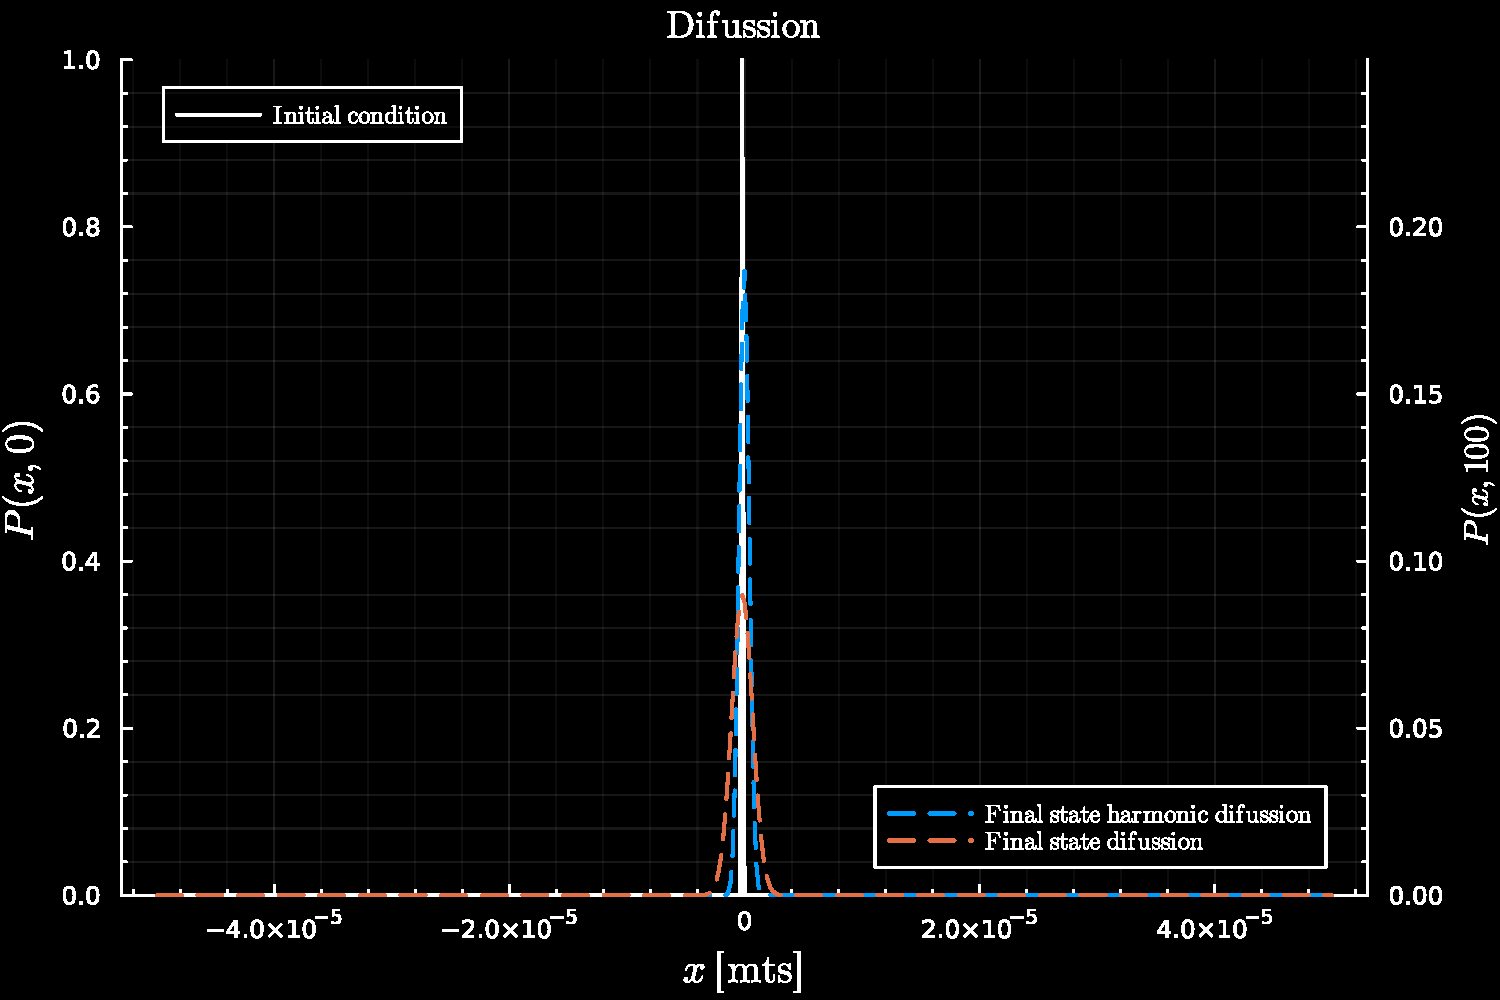
\includegraphics[width=0.8\textwidth]{imgs/hw8/difussionSols.pdf}
    \caption{Final state of the function at 100 temperal iterations of the system of diffusion and diffusion with harmonic potential.}
    \label{fig8:diffusionResults}
\end{figure}

\section{Wave propagation}

For the wave equation \eqref{eqn8:waveEquation}, all the second order derivatives where approximated using center finite differences scheme,
\begin{comment}
\begin{gather}
    \pdv[2]{u(x,y,t)}{t} = \upsilon(x,y)^2\qty[\pdv[2]{u(x,y,t)}{x} + \pdv[2]{u(x,y,t)}{y}],
\end{gather}

\begin{align*}
    \pdv[2]{u(x,y,t)}{t} &\approx \frac{u_{i,j}^{s+1} - 2u_{i,j}^s + u_{i,j}^{s-1}}{\Delta t ^2} \\
    \pdv[2]{u(x,y,t)}{x} &\approx \frac{u_{i+1,j}^{s} - 2u_{i,j}^s + u_{i-1,j}^{s}}{\Delta x ^2} \\
    \pdv[2]{u(x,y,t)}{y} &\approx \frac{u_{i,j+1}^{s} - 2u_{i,j}^s + u_{i,j-1}^{s}}{\Delta y ^2} 
\end{align*}
\end{comment}

\begin{align*}
    \frac{u_{i,j}^{s+1} - 2u_{i,j}^s + u_{i,j}^{s-1}}{\Delta t ^2} &= \upsilon_{i,j}^2\qty[\frac{u_{i+1,j}^s - 2u_{i,j}^s + u_{i-1,j}^s}{\Delta x ^2} + \frac{u_{i,j+1}^s - 2u_{i,j}^s + u_{i,j-1}^s}{\Delta y ^2}],
\end{align*}
and assuming that $\Delta r = \Delta x = \Delta y$,
\begin{gather*}
    u_{i,j}^{s+1} = \upsilon_{i,j}^2\frac{\Delta t^2}{\Delta r^2}\qty[\qty(u_{i+1,j}^s - 2u_{i,j}^s + u_{i-1,j}^s) + \qty(u_{i,j+1}^s - 2u_{i,j}^s + u_{i,j-1}^s)] + 2u_{i,j}^s - u_{i,j}^{s-1}.
\end{gather*}
As before, this equation can be implemented as a multiplication of matrices.
However it is important to acknowledge that this equation has two spatial dimensions, hence, the matrix multiplication established as before, needs to be applied for each other spatial node.
In other words, for each $x$ node a matrix multiplication to get the $y$ derivative is computed, and for each $y$ node the matrix multiplication to get the $x$ derivative is computed.

For numerical stability, the parameter $\upsilon\Delta t/\Delta r$ was set to $0.1$ and $\Delta x = 0.05$.
A point source, at the bottom right corner, was define as $10\sin\qty(0.5 t)$.
Finally, to introduce the wall of concrete as an impermeable material, the $\upsilon$ was define as a matrix of values of $0$ in the spatial nodes of the wall and $1$ in the rest of the matrix.

In figure \ref{fig8:waveResults} is the result of the propagation at 25 temporal units with the color-bar over saturated to increment the contrast of the oscillations.
In this figure it can be appreciated that wave at the source can permeate the hole room, except in side the wall as expected.
However, at the opposite corner with respect of the point source, the wave is more attenuated than the rest of the space.

\begin{figure}[ht!]
    \centering
    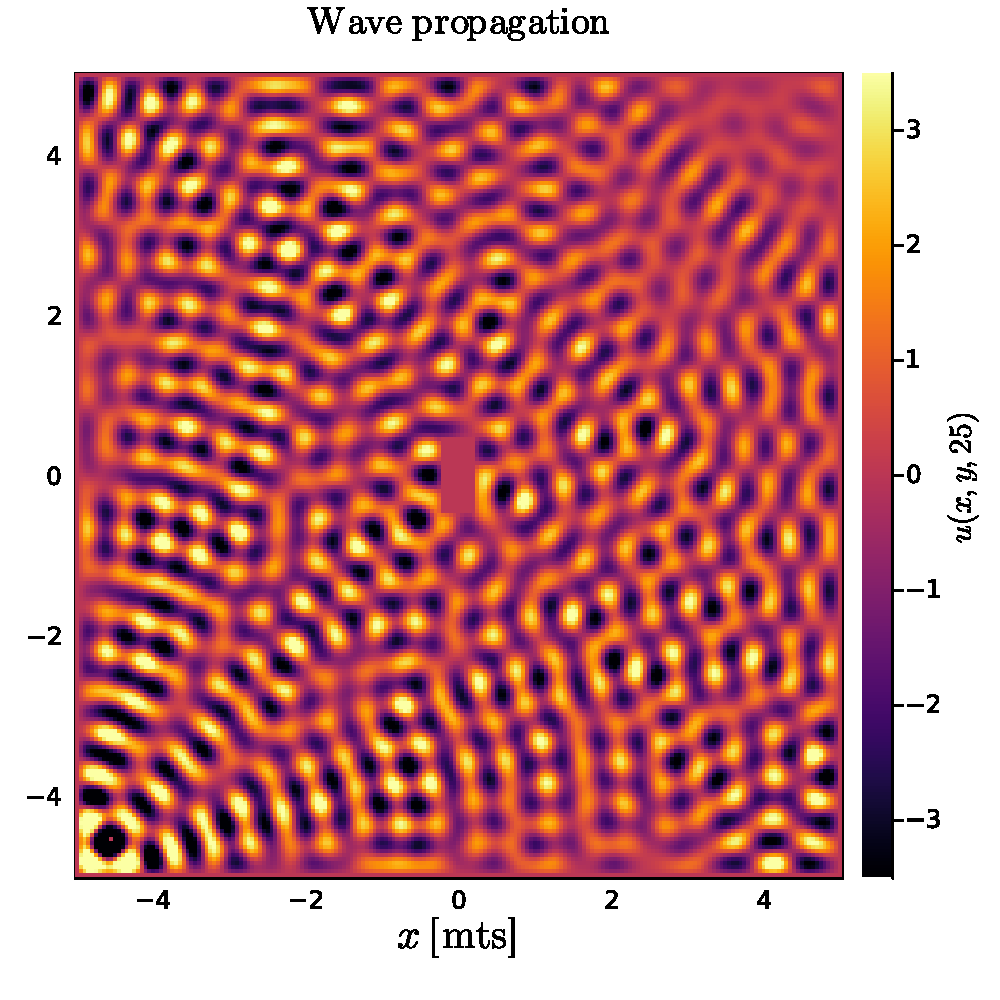
\includegraphics[width=0.8\textwidth]{imgs/hw8/waveEquationSols.pdf}
    \caption{Propagation of point source located at the bottom right corner of a room with perfect reflection at the boundaries.}
    \label{fig8:waveResults}
\end{figure}

% https://encyclopediaofmath.org/wiki/Absorbing_boundary_conditions
% https://www.sciencedirect.com/science/article/pii/S0165212511001491#f000005
% https://www.ams.org/journals/mcom/1977-31-139/S0025-5718-1977-0436612-4/S0025-5718-1977-0436612-4.pdf
% https://sci-hub.se/https://doi.org/10.2307/2008250

% https://math.mit.edu/classes/18.086/2006/am53.pdf

\end{document}